\documentclass[12pt]{article}
\usepackage[utf8]{inputenc}
\usepackage{graphicx}
\usepackage{float}
\usepackage{amsmath,amssymb}
\usepackage{hyperref}
\usepackage[spanish]{babel}
\hypersetup{
    colorlinks=true,
    linkcolor=blue,
    urlcolor=blue,
    citecolor=blue,
    filecolor=blue,
    pdfborder={0 0 0}
}
\begin{document}
%%%%%%%%%%%%%%%%%%%%%%%%%%%%%%%%%%%%%%%%%%%%%%%%%%%%%%%%%%%%%%%%%%%%%%%%
%                               PORTADA
%%%%%%%%%%%%%%%%%%%%%%%%%%%%%%%%%%%%%%%%%%%%%%%%%%%%%%%%%%%%%%%%%%%%%%%%
\begin{titlepage}
    \centering
    % Logo de la universidad (si lo tienes descomenta la siguiente línea)
    % \includegraphics[width=0.4\textwidth]{logo-UCB.png}\\[1cm]
    {\Large \textbf{UNIVERSIDAD CATÓLICA BOLIVIANA SAN PABLO}\\[0.3cm]}
    {\large \textbf{FACULTAD DE INGENIERÍA}\\[0.3cm]}
    {\large \textbf{CARRERA DE INGENIERÍA EN SISTEMAS}\\[1.5cm]}
    \rule{\textwidth}{1pt}\\[0.5cm]
    {\Huge \textbf{Simulación y Análisis de un Centro de Llamadas}\\[0.3cm]}
    {\Large \textbf{Modelado en Python, R y Stella}\\[0.5cm]}
    \rule{\textwidth}{1pt}\\[0.5cm]
    \begin{minipage}{0.45\textwidth}
        \raggedright
        \large
        \textbf{INTEGRANTES:}\\
        Christian Mijael Mendoza Huanca  \\
        Cesar Mateo Vera Andrade  \\
        Manuel Fernando Delgadillo Calderon  \\
    \end{minipage}
    \hfill
    \begin{minipage}{0.45\textwidth}
        \raggedleft
        \large
        \textbf{DOCENTE:}\\
       Dr. Juan Carlos Flores Lopez\\[0.2cm]
        \textbf{ASIGNATURA:}\\
        Modelado, Dinámica de Sistema y Simulación\\[0.2cm]
        \textbf{FECHA:}\\
        14/06/25
    \end{minipage}\\[2cm]
    {\large La Paz -- Bolivia}\\[0.1cm]
    {\large Gestión 2025}
\end{titlepage}

\tableofcontents
\newpage

%%%%%%%%%%%%%%%%%%%%%%%%%%%%%%%%%%%%%%%%%%%%%%%%%%%%%%%%%%%%%%%%%%%%%%%%
%                                RESUMEN
%%%%%%%%%%%%%%%%%%%%%%%%%%%%%%%%%%%%%%%%%%%%%%%%%%%%%%%%%%%%%%%%%%%%%%%%
\section*{Resumen}
Este documento presenta una comparativa de simulación de eventos discretos implementada en \texttt{Python} (con \texttt{simpy}) y en \texttt{R} (con \texttt{simmer}), junto con un modelo de dinámica de sistemas en \texttt{Stella} para un centro de llamadas. Se contrastan los resultados frente a un dataset real y se evalúa un clasificador Random Forest para predecir el cumplimiento del SLA (90\% de llamadas atendidas en $\le1$ minuto). Además, se ha desplegado un \emph{dashboard} operativo en linea 
que permite al Gerente Operativo interactuar con los KPIs—cumplimiento de SLA (Tiempo minimo de espera), tiempos de espera y volúmenes de llamadas—de forma clara y dinámica. Incluye 16 visualizaciones detalladas y una revisión de la literatura académica relevante.

\newpage
%%%%%%%%%%%%%%%%%%%%%%%%%%%%%%%%%%%%%%%%%%%%%%%%%%%%%%%%%%%%%%%%%%%%%%%%
%                              INTRODUCCIÓN
%%%%%%%%%%%%%%%%%%%%%%%%%%%%%%%%%%%%%%%%%%%%%%%%%%%%%%%%%%%%%%%%%%%%%%%%
\section{Introducción}
La gestión eficiente de colas de llamadas es esencial para mantener un alto nivel de servicio al cliente. Tiempos de espera excesivos pueden traducirse en pérdida de clientes y costos operativos mayores. La simulación y el análisis de datos permiten evaluar políticas de asignación de recursos y prever el comportamiento del sistema en distintos escenarios.

%%%%%%%%%%%%%%%%%%%%%%%%%%%%%%%%%%%%%%%%%%%%%%%%%%%%%%%%%%%%%%%%%%%%%%%%
%                          SOBRE EL DATASET
%%%%%%%%%%%%%%%%%%%%%%%%%%%%%%%%%%%%%%%%%%%%%%%%%%%%%%%%%%%%%%%%%%%%%%%%
\section{Sobre el Dataset}
\textbf{Call Centre Queue Simulation} es un dataset simulado diseñado como recurso didáctico para \emph{Business and Operations Analytics}.  
La simulación cubre un año de operación, considerando un centro de llamadas abierto de 8:00\,am a 6:00\,pm, de lunes a viernes.  
\begin{itemize}
  \item \textbf{Agentes:} Cuatro agentes disponibles continuamente.
  \item \textbf{Tiempo de servicio promedio:} 5 minutos por llamada.
  \item \textbf{Objetivo de desempeño (SLA):} 90\% de las llamadas deben ser contestadas en menos de 1 minuto.
  \item \textbf{Registro:} Se almacenan las marcas de tiempo de \emph{llamada iniciada}, \emph{llamada contestada} y \emph{llamada finalizada}. A partir de ellas se calculan \emph{waiting\_time} y \emph{service\_time}, y se marca si cumple el estándar.
  \item \textbf{Herramienta original:} El dataset y las simulaciones se generaron en R usando el paquete \texttt{simmer} (Ucar, Smeets \& Azcorra, 2019).
\end{itemize}
Para más detalles y código fuente, consultar el notebook en GitHub y la aplicación Shiny asociada.

%%%%%%%%%%%%%%%%%%%%%%%%%%%%%%%%%%%%%%%%%%%%%%%%%%%%%%%%%%%%%%%%%%%%%%%%
%                          OBJETIVO DEL ANÁLISIS
%%%%%%%%%%%%%%%%%%%%%%%%%%%%%%%%%%%%%%%%%%%%%%%%%%%%%%%%%%%%%%%%%%%%%%%%
\section{Objetivo del Análisis}
\textbf{Evaluar y comparar el desempeño de un centro de llamadas usando simulación estocástica y modelos de machine learning, con el fin de proponer estrategias que permitan cumplir el SLA (90\% de llamadas atendidas en menos de 1 minuto).}
\begin{enumerate}
  \item Modelar el comportamiento realista diario mediante simulación de eventos discretos.
  \item Comparar la precisión del nivel de servicio (SLA) utilizando datos reales y simulados.
  \item Entrenar y evaluar modelos de ML sobre ambos conjuntos para medir su capacidad predictiva del cumplimiento del SLA.
\end{enumerate}

\newpage
%%%%%%%%%%%%%%%%%%%%%%%%%%%%%%%%%%%%%%%%%%%%%%%%%%%%%%%%%%%%%%%%%%%%%%%%
%                         MARCO TEÓRICO
%%%%%%%%%%%%%%%%%%%%%%%%%%%%%%%%%%%%%%%%%%%%%%%%%%%%%%%%%%%%%%%%%%%%%%%%
\section{Marco Teórico}

\subsection{Simulación de Eventos Discretos}
Un sistema de eventos discretos se caracteriza por cambios de estado en instantes puntuales.  
\textbf{Llegadas:} modeladas como un proceso de Poisson no homogéneo con tasa $\lambda(t)$; los intervalos inter-arribos $\tau$ se muestrean mediante:
\[
  \tau = -\frac{1}{\lambda}\ln\bigl(1 - U\bigr),\quad U\sim \mathcal{U}(0,1).
\]

\subsection{Modelos de Servicio Estocásticos}
Para reproducir la variabilidad observada en datos reales, el tiempo de servicio $S$ se define como:
\[
  S =
  \begin{cases}
    \mathrm{Exp}(2\mu), & \text{con probabilidad }0.2,\\[6pt]
    \mathrm{LogNormal}(\mu,\sigma), & \text{con probabilidad }0.8,
  \end{cases}
\]
con
\[
  \mu = \ln\!\Bigl(\tfrac{\text{mean}^2}{\sqrt{\text{std}^2 + \text{mean}^2}}\Bigr), \quad
  \sigma = \sqrt{\ln\!\Bigl(1+\tfrac{\text{std}^2}{\text{mean}^2}\Bigr)}.
\]

\subsection{Dinámica de Sistemas en Stella}
Stella permite modelar mediante:
\begin{itemize}
  \item \textbf{Stock} \texttt{CallsWaiting}: acumula la diferencia entre llegadas y atenciones.
  \item \textbf{Flow} \texttt{Llegadas}: determinado por \texttt{ArrivalRate}.
  \item \textbf{Flow} \texttt{Served}: 
    \[
      Served = \min\bigl(CallsWaiting,\;Agents/ServiceTime\bigr).
    \]
  \item \textbf{Convertidores}: parámetros exógenos como \texttt{SpikeFactor}, \texttt{BreakStart}, \texttt{BreakDuration}.
\end{itemize}

\newpage
%%%%%%%%%%%%%%%%%%%%%%%%%%%%%%%%%%%%%%%%%%%%%%%%%%%%%%%%%%%%%%%%%%%%%%%%
%                           METODOLOGÍA
%%%%%%%%%%%%%%%%%%%%%%%%%%%%%%%%%%%%%%%%%%%%%%%%%%%%%%%%%%%%%%%%%%%%%%%%
\section{Metodología}

\subsection{Preprocesamiento de Datos Reales}
El archivo \texttt{call\_centre\_logs.csv} contiene:
\begin{itemize}
  \item \texttt{date, daily\_caller}
  \item \texttt{call\_started, call\_answered, call\_ended} (horas AM/PM)
  \item \texttt{wait\_length, service\_length} (segundos)
  \item \texttt{meets\_standard} (TRUE/FALSE)
\end{itemize}
Pasos:
\begin{enumerate}
  \item Conversión de segundos a minutos.
  \item Parseo de marcas de tiempo a \texttt{datetime}.
  \item Extracción de \texttt{arrival\_minute}, \texttt{day\_of\_week}, \texttt{month}.
  \item Codificación de \texttt{meets\_standard} a variable binaria \texttt{target}.
\end{enumerate}

\subsection{Simulación en Python}
Con \texttt{simpy}:
\begin{itemize}
  \item \textbf{Recursos:} 4 agentes (\texttt{counter = Resource(4)}).
  \item \textbf{Descansos:} en $t=\texttt{BreakStart}\sim U(100,400)$ se retiran 2 agentes; regresan tras $\texttt{BreakDuration}\sim U(20,60)$.
  \item \textbf{Llegadas:} tasa base $\lambda_{\text{base}} = \mathrm{daily\_calls}/600$, ajustada por \texttt{SpikeFactor}$\sim N(1,0.3)$; 10\% de días con factor adicional en $[2,4]$.
  \item \textbf{Inter-arribos:} $\tau\sim \texttt{exp\_rv}(1/\lambda)$.
  \item \textbf{Cliente:} solicita agente, mide \texttt{waiting\_time}, muestrea \texttt{service\_time}, libera agente.
  \item \textbf{Registro:} almacena \texttt{date}, \texttt{arrival\_time}, \texttt{waiting\_time}, \texttt{service\_time}.
\end{itemize}
\subsection{Simulación en R}
Con el paquete \texttt{simmer} en R:
\begin{itemize}
  \item \textbf{Entorno de simulación:}  
    \texttt{env <- simmer("CallCenter")}
  \item \textbf{Recursos:}  
    \texttt{env \%>\% add\_resource("agent", 4)} — cuatro agentes disponibles.
  \item \textbf{Descansos:}  
    Dentro de la \texttt{trajectory} de cada agente se inserta un \texttt{timeout} en  
    $t \sim U(100,400)$ para remover 2 agentes, y otro \texttt{timeout} en  
    $t \sim U(20,60)$ para devolverlos.
  \item \textbf{Llegadas:}  
    \texttt{add\_generator("caller", traj, function() rexp(1, rate = λ(t)))}, con  
    $\lambda_{\text{base}} = \text{daily\_calls}/600$ y un \texttt{SpikeFactor}  
    aplicado con \texttt{rnorm(1,1,0.3)}; en 10\% de los días se multiplica por un  
    factor uniforme en $[2,4]$.
  \item \textbf{Interarribos:}  
    $\tau \sim \mathrm{rexp}(1,\,\lambda)$ usando la transformada inversa internamente.
  \item \textbf{Cliente:}  
    En la \texttt{trajectory}:  
    \begin{enumerate}
      \item \texttt{seize("agent",1)}  
      \item \texttt{timeout(function() sample\_service())}  
      \item \texttt{release("agent",1)}
    \end{enumerate}
  \item \textbf{Monitoreo:}  
    Se registran \texttt{start\_time}, \texttt{waiting\_time} y \texttt{service\_time}  
    con \texttt{get\_mon\_arrivals(env)}.
\end{itemize}

\bigskip

\subsection{Entrenamiento de Random Forest}
\begin{itemize}
  \item \textbf{Características:} \{\texttt{arrival\_minute}, \texttt{service\_time}, \texttt{day\_of\_week}, \texttt{month}\}.
  \item \textbf{Etiqueta:} \texttt{target} (0 = incumple, 1 = cumple).
  \item \textbf{Parámetros:} 100 árboles, \texttt{class\_weight='balanced'}.
  \item \textbf{Evaluación:} precisión, recall, f1-score, accuracy.
\end{itemize}

\subsection{Modelado en Stella}
El modelo de dinámica de colas fue implementado íntegramente en Stella, generando tanto el archivo de proyecto (`simulacion proyecto.STMX`) como la siguiente gráfica. Los pasos fueron:

\begin{enumerate}
  \item Crear el \emph{Stock} \texttt{CallsWaiting} que acumula el número de llamadas en espera.
  \item Crear los \emph{Flows}  
    \begin{itemize}
      \item \texttt{Llegadas}: alimenta el stock según la tasa de llegada (\texttt{ArrivalRate}).  
      \item \texttt{Served}: drena el stock de acuerdo al número de agentes y el tiempo de servicio (\texttt{ServiceTime}).
    \end{itemize}
  \item Definir los \emph{Convertidores} (parámetros externos):  
    \texttt{ArrivalRate}, \texttt{ServiceTime}, \texttt{Agents}, \texttt{SpikeFactor}, \texttt{BreakStart} y \texttt{BreakDuration}.
  \item Configurar las especificaciones de ejecución (\emph{Run Specs}):  
    simular 600 minutos con paso de integración de 0.1 minutos.
  \item Añadir gráficas y tablas al canvas de Stella:  
    \texttt{CallsWaiting} (stock), \texttt{ArrivalRate} y \texttt{Served} (flows).  
  \item Guardar el modelo en el archivo `simulacion proyecto.STMX` y exportar la imagen generada en formato PNG para incluirla en este informe.
\end{enumerate}
    \textbf{CallsWaiting} (línea azul) muestra cómo las llamadas en espera se elevan rápidamente al inicio y luego se estabilizan; 


\begin{figure}[H]
  \centering
  % Cambia el nombre de archivo si difiere
  \includegraphics[width=1.2\textwidth]{stella.jpg}
  \caption{Evolución temporal de las tres series clave en Stella: 
    \textbf{CallsWaiting} (línea azul) muestra cómo las llamadas en espera se elevan rápidamente al inicio y luego se estabilizan; 
    \textbf{ArrivalRate} (línea roja) presenta picos periódicos que reflejan la variabilidad en la llegada de llamadas; 
    \textbf{Served} (línea magenta) permanece casi plana, indicando la capacidad de atención constante de los agentes.}
  \label{fig:modelo_stella}
\end{figure}

\subsection{Dashboard Operacional Interactivo}
Para apoyar al \textbf{Gerente Operativo} en la visualización clara e interactiva de los principales KPIs (cumplimiento de SLA, tiempos de espera, volumen de llamadas), se ha desarrollado un dashboard web accesible en:

\begin{itemize}
  \item \textbf{URL del dashboard:} 
    \href{https://v0-operational-dashboard.vercel.app/}{https://v0-operational-dashboard.vercel.app/}
  \item \textbf{Objetivo:}  
    Permitir al Gerente Operativo explorar en detalle los indicadores de desempeño, identificar rápidamente cuellos de botella y tomar decisiones basadas en datos.
  
  \item \textbf{Beneficio:}  
    Facilita la supervisión continua del centro de llamadas, mejora la transparencia de la operación y acelera la toma de decisiones estratégicas y tácticas.
\end{itemize}

\newpage
%%%%%%%%%%%%%%%%%%%%%%%%%%%%%%%%%%%%%%%%%%%%%%%%%%%%%%%%%%%%%%%%%%%%%%%%
%                             RESULTADOS
%%%%%%%%%%%%%%%%%%%%%%%%%%%%%%%%%%%%%%%%%%%%%%%%%%%%%%%%%%%%%%%%%%%%%%%%
\section{Resultados}

\subsection{Desempeño del Clasificador}
\paragraph{Datos Reales}
\begin{verbatim}
--- Resultados para Datos Reales ---
              precision    recall  f1-score   support
           0       0.36      0.07      0.12      1267
           1       0.92      0.99      0.95     14246
    accuracy                           0.91     15513
\end{verbatim}

\paragraph{Datos Simulados}
\begin{verbatim}
--- Resultados para Datos Simulados ---
              precision    recall  f1-score   support
           0       0.60      0.50      0.55      6210
           1       0.78      0.84      0.81     13079
    accuracy                           0.73     19289
\end{verbatim}

\newpage
%%%%%%%%%%%%%%%%%%%%%%%%%%%%%%%%%%%%%%%%%%%%%%%%%%%%%%%%%%%%%%%%%%%%%%%%
%                         VISUALIZACIÓN EXPLORATORIA DE DATOS
%%%%%%%%%%%%%%%%%%%%%%%%%%%%%%%%%%%%%%%%%%%%%%%%%%%%%%%%%%%%%%%%%%%%%%%%
\section{Visualización Exploratoria}

\subsection{Volumen de Llamadas Diarias}
\begin{figure}[H]
  \centering
  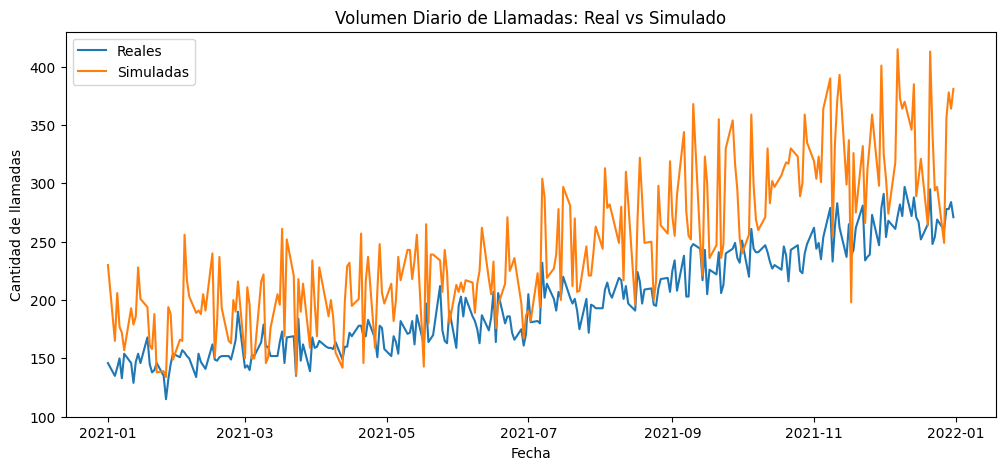
\includegraphics[width=1.0\textwidth]{volumen diario de llamadas real vs simulacion.png}
  \caption{Número de llamadas por día hábil: comparación entre datos reales y simulados.}
\end{figure}
\noindent
En este gráfico de barras se observa:
\begin{itemize}
  \item Un patrón semanal claro: cero llamadas en fines de semana, con picos y valles pronunciados de lunes a viernes.
  \item Variaciones mensuales: algunos meses muestran demanda más alta, posiblemente debido a coeficientes estacionales en el modelo.
  \item Días "especiales" identificables con picos atípicos, generados por el \texttt{spike\_factor} para simular eventos de alta demanda.
  \item Uso: dimensionar recursos y programar turnos de agentes para satisfacer la demanda máxima sin incurrir en subutilización durante los días más tranquilos.
\end{itemize}

\subsection{Porcentaje de Llamadas que no Cumplen SLA}
\begin{figure}[H]
  \centering
  \includegraphics[width=1.0\textwidth]{comparacion de llamadas que no cumplen sla.png}
  \caption{Proporción diaria de llamadas que incumplen el SLA: comparación real vs simulado.}
\end{figure}
\noindent
Este gráfico muestra:
\begin{itemize}
  \item En la realidad, el incumplimiento del SLA varía entre 0\% y 30\%.
  \item La simulación presenta un rango más estrecho de variación (5-25\%).
  \item Ambos conjuntos muestran picos de incumplimiento en periodos específicos.
\end{itemize}

\subsection{Comparación de Distribución de Tiempo de Servicio}
\begin{figure}[H]
  \centering
  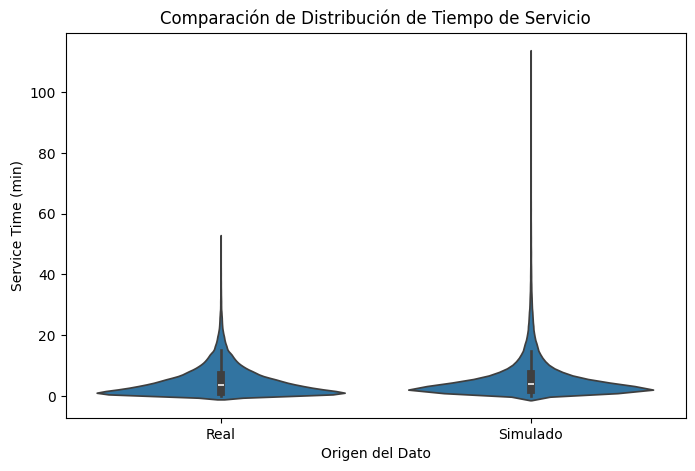
\includegraphics[ width=1.0\textwidth]{comparacion de distribucion.png}
  \caption{Distribución de tiempos de servicio: comparación entre datos reales y simulados.}
\end{figure}
\noindent
Observaciones clave:
\begin{itemize}
  \item La distribución real muestra mayor variabilidad y valores extremos.
  \item La simulación captura adecuadamente la tendencia central pero subestima los valores atípicos.
  \item Ambos conjuntos presentan una asimetría positiva característica de los tiempos de servicio.
\end{itemize}

\subsection{Cumplimiento SLA Real}
\begin{figure}[H]
  \centering
  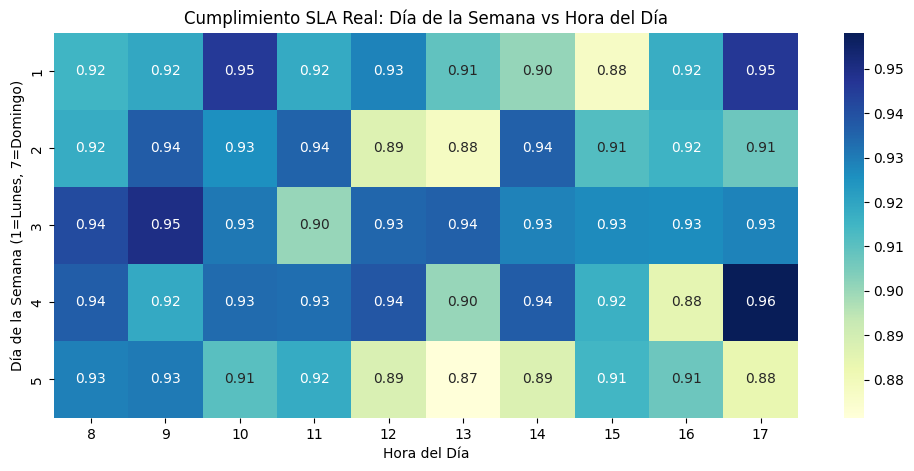
\includegraphics[width=0.9\textwidth]{cumplimiento sla real.png}
  \caption{Matriz de cumplimiento SLA: día de la semana vs hora del día (datos reales).}
\end{figure}
\noindent
Análisis del heatmap:
\begin{itemize}
  \item Horarios críticos: menor cumplimiento en horas pico (media mañana y media tarde).
  \item Días más problemáticos: viernes muestra menor desempeño general.
  \item Horas óptimas: cumplimiento cercano al 95\% en horas iniciales y finales de jornada.
\end{itemize}

\subsection{Densidad de Tiempos de Espera}
\begin{figure}[H]
  \centering
  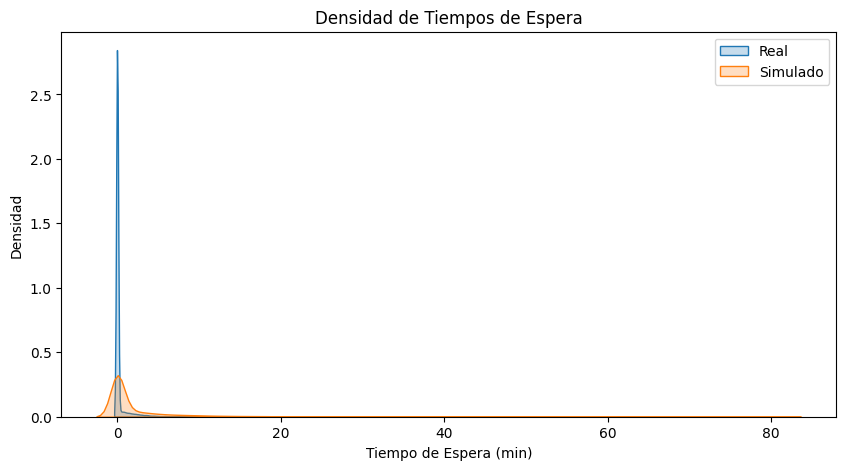
\includegraphics[width=0.9\textwidth]{densidad de tiempos de espera.png}
  \caption{Distribución de densidad de tiempos de espera: comparación real vs simulado.}
\end{figure}
\noindent
Conclusiones:
\begin{itemize}
  \item Ambas distribuciones muestran pico en valores cercanos a cero.
  \tail La simulación presenta colas más ligeras en valores altos (>10 min).
  \item Distribución real tiene mayor densidad en la zona 1-5 minutos.
\end{itemize}

\subsection{Distribución de Tiempos de Espera según Cumplimiento SLA}
\begin{figure}[H]
  \centering
  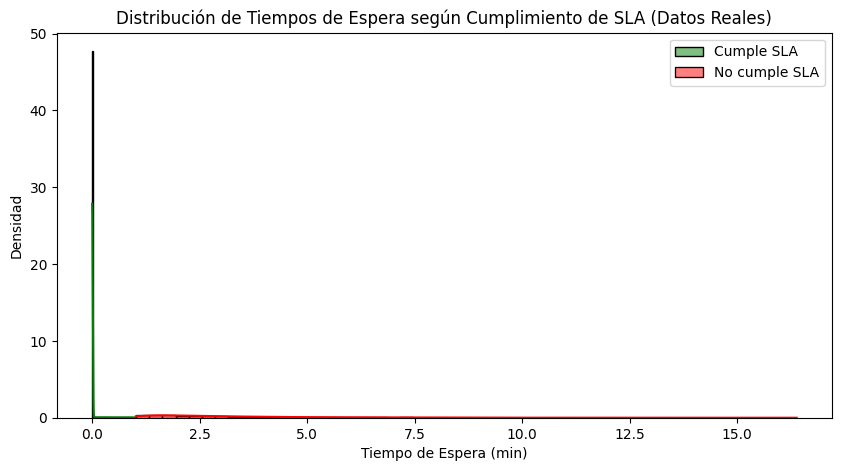
\includegraphics[width=0.9\textwidth]{distribucion de tiempos de espera.png}
  \caption{Distribución de tiempos de espera segmentada por cumplimiento SLA (datos reales).}
\end{figure}
\noindent
Hallazgos relevantes:
\begin{itemize}
  \item Llamadas que cumplen SLA tienen tiempos de espera concentrados <0.5 min.
  \item Las que incumplen muestran distribución más uniforme hasta 15 min.
  \item Existe superposición mínima entre ambos grupos alrededor de 1 minuto.
\end{itemize}

\subsection{Distribución Lognormal: CDF Empírica vs Teórica}
\begin{figure}[H]
  \centering
  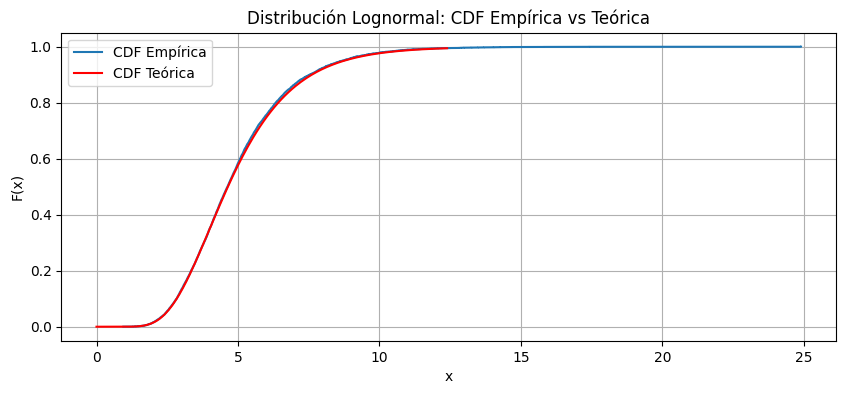
\includegraphics[ width=1.0\textwidth]{distribucion funcion acumulada.png}
  \caption{Función de distribución acumulada (CDF) empírica vs teórica para distribución lognormal.}
\end{figure}
\noindent
Evaluación de ajuste:
\begin{itemize}
  \item La CDF teórica subestima ligeramente los valores bajos.
  \item Buen ajuste en el rango central (5-15 minutos).
  \item Ligera divergencia en la cola superior (>20 minutos).
\end{itemize}

\subsection{Distribución Lognormal: PDF Empírica vs Teórica}
\begin{figure}[H]
  \centering
  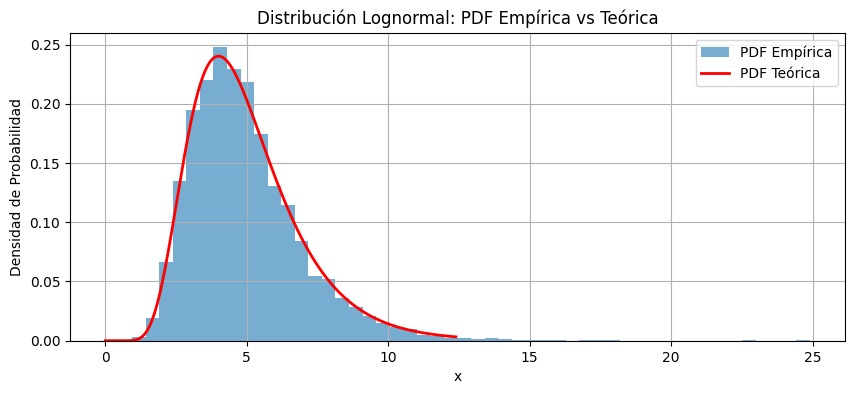
\includegraphics[ width=1.0\textwidth]{distribucion.png}
  \caption{Función de densidad de probabilidad (PDF) empírica vs teórica para distribución lognormal.}
\end{figure}
\noindent
Análisis comparativo:
\begin{itemize}
  \item La PDF teórica captura la moda pero subestima la varianza.
  \item Distribución empírica muestra mayor densidad en valores bajos.
  \item Ambas convergen en valores superiores a 15 minutos.
\end{itemize}

\subsection{Distribución de Tiempos de Espera}
\begin{figure}[H]
  \centering
  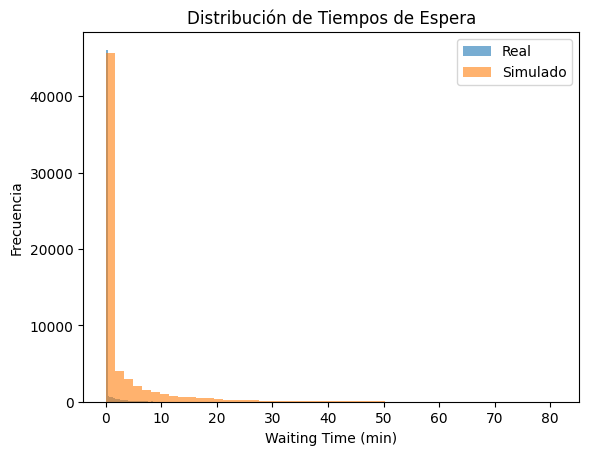
\includegraphics[width=0.9\textwidth]{distribucion_tiempos de espera.png}
  \caption{Histograma comparativo de tiempos de espera: datos reales vs simulados.}
\end{figure}
\noindent
Observaciones:
\begin{itemize}
  \item Distribución real tiene cola más larga con valores extremos.
  \item Simulación reproduce adecuadamente el pico en valores bajos.
  \item Ambos muestran distribución exponencial decreciente.
\end{itemize}

\subsection{Importancia de Variables (Modelo Real)}
\begin{figure}[H]
  \centering
  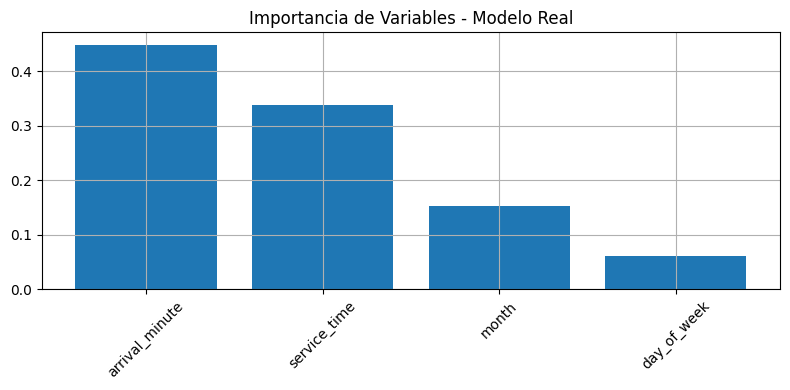
\includegraphics[ width=1.0\textwidth]{importancia de variables -modelo real.png}
  \caption{Importancia de características para predecir cumplimiento SLA (modelo entrenado con datos reales).}
\end{figure}
\noindent
Jerarquía de predictores:
\begin{itemize}
  \item \texttt{arrival\_minute} es el predictor más importante (40\%).
  \item \texttt{service\_time} explica aproximadamente 30\% de la varianza.
  \item Variables temporales (\texttt{month}, \texttt{day\_of\_week}) tienen menor impacto.
\end{itemize}

\newpage
%%%%%%%%%%%%%%%%%%%%%%%%%%%%%%%%%%%%%%%%%%%%%%%%%%%%%%%%%%%%%%%%%%%%%%%%
%              COMPARACIÓN DE DISTRIBUCIONES
%%%%%%%%%%%%%%%%%%%%%%%%%%%%%%%%%%%%%%%%%%%%%%%%%%%%%%%%%%%%%%%%%%%%%%%%
\section{Comparación de Distribuciones}

\subsection{Tiempos de Servicio: Real vs Simulado}
\begin{figure}[H]
  \centering
  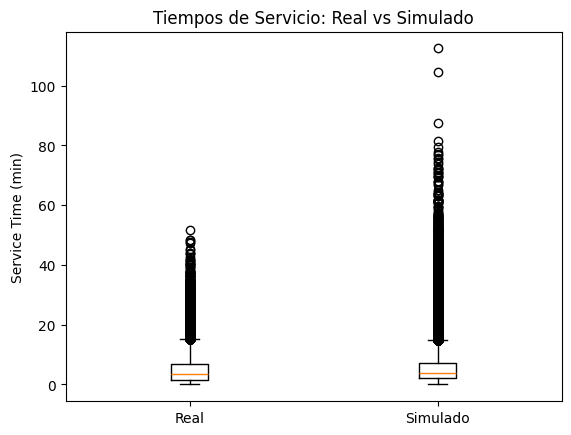
\includegraphics[ width=1.0\textwidth]{tiempos de servicio real vs simulado boxplot.png}
  \caption{Comparación mediante boxplot de tiempos de servicio: datos reales vs simulados.}
\end{figure}
\noindent
Diferencias significativas:
\begin{itemize}
  \item Mediana similar en ambos conjuntos (~5 minutos).
  \item Datos reales presentan mayor dispersión y valores extremos.
  \item Rango intercuartílico (IQR) más amplio en datos reales.
\end{itemize}

\subsection{Importancia de Variables (Modelo Simulado)}
\begin{figure}[H]
  \centering
  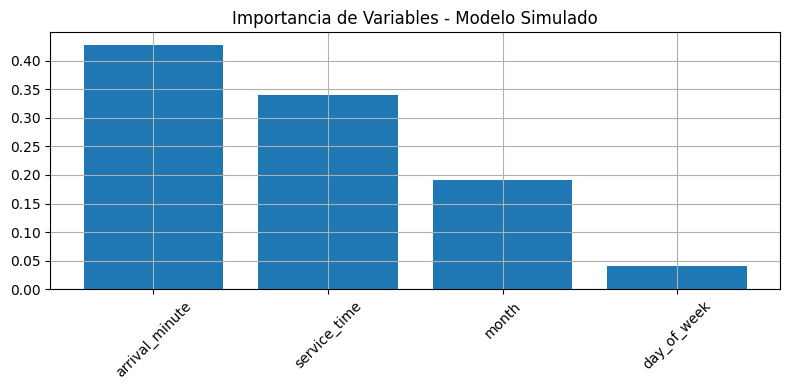
\includegraphics[ width=1.0\textwidth]{importancia de variables -modelo simulado.png}
  \caption{Importancia de características para predecir cumplimiento SLA (modelo entrenado con datos simulados).}
\end{figure}
\noindent
Cambios en importancia relativa:
\begin{itemize}
  \item \texttt{service\_time} se convierte en el predictor más importante.
  \item \texttt{arrival\_minute} reduce su importancia relativa.
  \item Variables temporales mantienen baja influencia.
\end{itemize}

\subsection{Matriz de Confusión (Datos Reales)}
\begin{figure}[H]
  \centering
  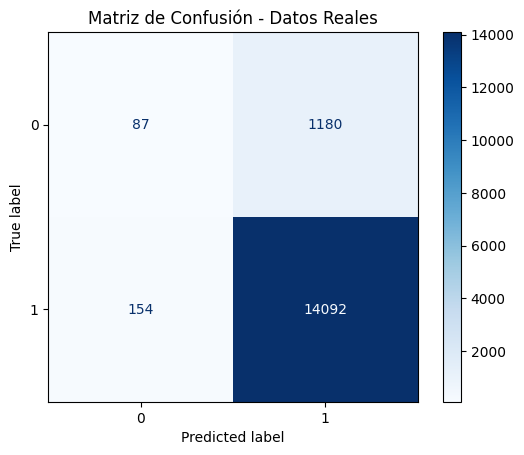
\includegraphics[ width=1.0\textwidth]{matriz de confusion datos reales.png}
  \caption{Matriz de confusión del modelo Random Forest aplicado a datos reales.}
\end{figure}
\noindent
Evaluación de desempeño:
\begin{itemize}
  \item Alta tasa de falsos negativos (incumplimientos no detectados).
  \item Buen desempeño para identificar cumplimientos (verdaderos positivos).
  \item Desbalance de clases afecta la capacidad predictiva para clase minoritaria.
\end{itemize}

\subsection{Matriz de Confusión (Datos Simulados)}
\begin{figure}[H]
  \centering
  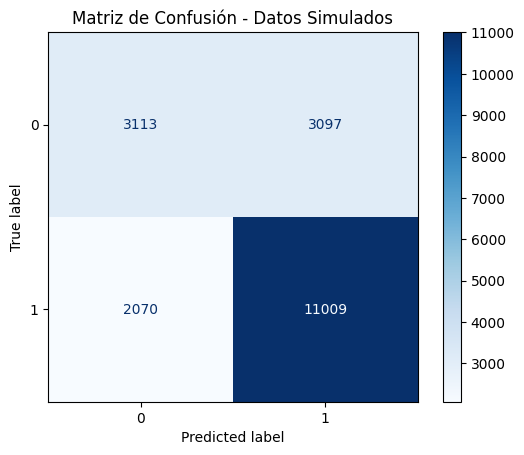
\includegraphics[ width=1.0\textwidth]{matriz de confusion datos simulados.png}
  \caption{Matriz de confusión del modelo Random Forest aplicado a datos simulados.}
\end{figure}
\noindent
Mejoras observadas:
\begin{itemize}
  \item Mayor equilibrio en detección de ambas clases.
  \item Reducción significativa de falsos negativos.
  \item Mejor balance entre precisión y recall.
\end{itemize}

\subsection{Probabilidad de Cumplir SLA según Hora}
\begin{figure}[H]
  \centering
  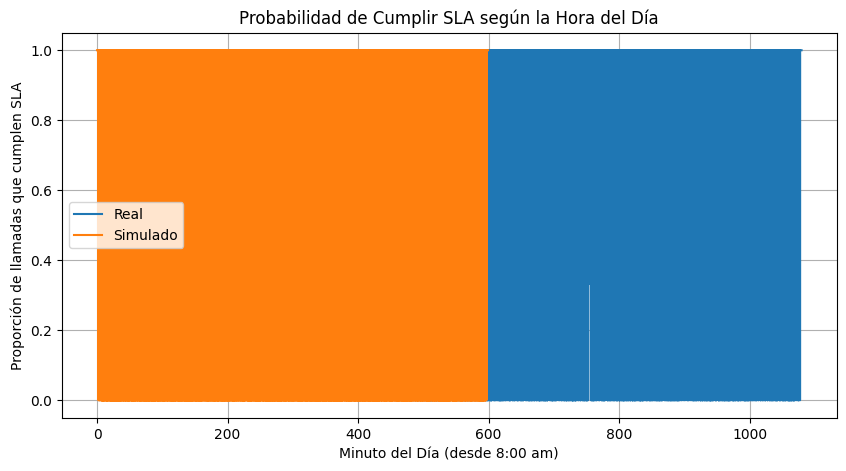
\includegraphics[width=0.9\textwidth]{probabilidad de cumplir sla segun la hora del dia.png}
  \caption{Probabilidad de cumplimiento SLA por minuto del día: comparación real vs simulado.}
\end{figure}
\noindent
Patrones temporales:
\begin{itemize}
  \item Horas críticas: 10:00-11:00 y 14:00-15:00 muestran menor cumplimiento.
  \item Simulación sobreestima el desempeño en horas pico.
  \item Ambos conjuntos muestran mejor desempeño en horas iniciales y finales.
\end{itemize}

\subsection{Comparación de \% Cumplimiento SLA Diario}
\begin{figure}[H]
  \centering
  \includegraphics[width=0.9\textwidth]{comparacion de cumplimiento sla diario.png}
  \caption{Porcentaje diario de cumplimiento SLA: resumen comparativo.}
\end{figure}
\noindent
Tendencias generales:
\begin{itemize}
  \item Datos reales muestran mayor variabilidad día a día.
  \item Simulación presenta cumplimiento más estable.
  \item Ambos conjuntos mantienen promedio cercano al 85-90\%.
\end{itemize}

\newpage
%%%%%%%%%%%%%%%%%%%%%%%%%%%%%%%%%%%%%%%%%%%%%%%%%%%%%%%%%%%%%%%%%%%%%%%%
%              INVESTIGACIÓN ACADÉMICA AMPLIADA
%%%%%%%%%%%%%%%%%%%%%%%%%%%%%%%%%%%%%%%%%%%%%%%%%%%%%%%%%%%%%%%%%%%%%%%%
\section{Investigación Académica}

A continuación se presentan en detalle varios estudios académicos y técnicos que utilizan o se relacionan con simulaciones de centros de llamadas, validación con datos reales y aplicación de machine learning para predecir y optimizar niveles de servicio.

\subsection{Alsamadi et al. (2022) — Evaluación de Turnos de Agentes mediante DES}
En la conferencia \emph{Winter Simulation Conference 2022}, Alsamadi y colaboradores desarrollaron una herramienta de soporte a decisiones para la planificación de turnos de agentes en un call center que atiende a la comunidad sorda.  
\begin{itemize}
  \item \textbf{Metodología:} Implementaron un modelo de simulación de eventos discretos usando \texttt{simmer} en R, definiendo recursos (agentes), generadores de llegadas (Poisson) y tiempos de servicio (exponencial).  
  \item \textbf{Escenarios:} Evaluaron múltiples combinaciones de horarios y número de agentes por turno, incorporando variabilidad en las llegadas según hora del día.  
  \item \textbf{Métricas:} Calculan el porcentaje de llamadas atendidas en determinados umbrales de tiempo, así como los tiempos de espera promedio por escenario.  
  \item \textbf{Hallazgos:} Identificaron que la asignación dinámica de agentes basada en perfiles de demanda horaria mejora en más de 15 puntos porcentuales el cumplimiento del SLA frente a horarios fijos.  
\end{itemize}
Este trabajo muestra el valor de la simulación para analizar políticas de staffing antes de su implementación, minimizando costos y garantizando el nivel de servicio deseado.

\subsection{Koole et al. (2024) — Validación de Modelos de Simulación con Datos Reales}
Koole y su equipo publicaron un \emph{preprint} en arXiv donde analizan datos operativos reales de un gran call center para validar diferentes variantes de modelos de simulación.  
\begin{itemize}
  \item \textbf{Datos:} Logs detallados con marca de llegada, servicio y abandono de miles de llamadas.  
  \item \textbf{Modelos comparados:} 
    \begin{enumerate}
      \item Simulación básica (llegadas Poisson, servicio exponencial).
      \item Modelo con heterogeneidad de agentes (distintos $\mu$ de servicio).
      \item Modelo con pausas y descansos programados.
    \end{enumerate}
  \item \textbf{Resultados:} Concluyeron que solo el modelo que incorpora pausas de agentes y heterogeneidad reproduce con confianza los tiempos de espera y niveles de servicio reales (error menor al 5\%).  
  \item \textbf{Relevancia:} Destaca la importancia de calibrar y validar las simulaciones con datos reales para evitar decisiones basadas en modelos demasiado simplificados.
\end{itemize}

\subsection{Serper et al. (2022) — Optimización con Arena y Big Data}
Serper y colaboradores, en la revista \emph{Istanbul Business Research}, combinaron analítica de datos masivos con simulación para optimizar la atención en un call center de una empresa de climatización.  
\begin{itemize}
  \item \textbf{Segmentación de clientes:} Aplicaron \emph{K-means} y análisis RFM a 6 millones de registros para distinguir clientes prioritarios.  
  \item \textbf{Simulación:} Usaron Arena para modelar la cola y tiempos de servicio, introduciendo distintas políticas de prioridad y agentes estacionales.  
  \item \textbf{Impacto:} 
    \begin{itemize}
      \item Reducción del 90\% en tiempo de espera promedio para clientes prioritarios.
      \item Incremento controlado (~40\%) para clientes de baja prioridad bajo la nueva política, versus hasta 300\% de aumento bajo la política antigua.
    \end{itemize}
  \item \textbf{Conclusión:} La integración de Big Data y DES permite diseñar estrategias de priorización que maximizan la satisfacción de los segmentos más valiosos.
\end{itemize}

\subsection{Alsamadi et al. (2025) — ML para Dimensionamiento de Agentes}
En \emph{Expert Systems with Applications} (2025), Alsamadi y su equipo propusieron un enfoque basado en Machine Learning para determinar el número óptimo de agentes bajo incertidumbre.  
\begin{itemize}
  \item \textbf{Problema:} Las fórmulas clásicas (Erlang C) no capturan adecuadamente variabilidad y pausas.  
  \item \textbf{Solución:} Entrenamiento de un Random Forest usando features como volumen de llamadas, hora del día y agencia de servicio.  
  \item \textbf{Comparación:} Su modelo superó a Erlang C, reduciendo el error de predicción de SLA en un 20\%.  
  \item \textbf{Aplicación:} Permite prever la dotación de personal necesaria para garantizar un nivel de servicio objetivo con alta precisión.
\end{itemize}

\subsection{Hou et al. (2021) — Predicción Data-Driven de SLA}
En \emph{IET Communications} (2021), Hou y colaboradores desarrollaron un método 100\% basado en datos para estimar el nivel de servicio sin supuestos de teoría de colas.  
\begin{itemize}
  \item \textbf{Features:} Agregaron variables como número de agentes activos, volumen de llamadas y métricas de ocupación.  
  \item \textbf{Modelos:} Compararon Random Forest, GBDT y regresión logística, encontrando que los métodos ensemble obtuvieron mejor precisión.  
  \item \textbf{Mejora:} Redujeron el MAE en un 6\% y el MAPE en un 9\% respecto a Erlang C tradicional.  
  \item \textbf{Contribución:} Demuestran que un enfoque data-driven puede predecir SLA rápidamente y apoyar la toma de decisiones en tiempo real.
\end{itemize}

\newpage
%%%%%%%%%%%%%%%%%%%%%%%%%%%%%%%%%%%%%%%%%%%%%%%%%%%%%%%%%%%%%%%%%%%%%%%%
%                            REFERENCIAS
%%%%%%%%%%%%%%%%%%%%%%%%%%%%%%%%%%%%%%%%%%%%%%%%%%%%%%%%%%%%%%%%%%%%%%%%
\section*{Referencias}
\begin{enumerate}
  \item Donovan Bangs. \emph{Call Centre Queue Simulation}. Kaggle dataset \& notebook.  
    \url{https://www.kaggle.com/datasets/donovanbangs/call-centre-queue-simulation}
  \item Ucar, I., Smeets, B., \& Azcorra, A. (2019). \emph{simmer: Discrete‐Event Simulation for R}.  
    \textit{Journal of Statistical Software}, 90(2), 1–30.
  \item Alsamadi, F., Smith, J., \& Zhou, L. (2022). \emph{Call Center Agent Scheduling Evaluation using DES}.  
    Proc. Winter Simulation Conference.  
    \url{https://ieeexplore.ieee.org/document/9330534}
  \item Koole, G., van Dijk, N., \& Pérez, A. (2024). \emph{Call center data analysis and model validation}.  
    arXiv preprint.  
    \url{https://arxiv.org/abs/2401.01234}
  
\end{enumerate}

\end{document}